% =============================================================================
% CHAPTER 21: DYNAMIC PORTFOLIO EVOLUTION
% =============================================================================
%------------------------------------------------------------------------------
% Chapter 21: Dynamic Portfolio Evolution - When and How to Redesign
%------------------------------------------------------------------------------
% Version: 1.0 (January 2026) - New chapter from refactored Ch20 dynamic content
%
% Purpose: Extend Chapter 20's static portfolio design theory to DYNAMIC settings
% where Status Quo S_t evolves over time. Focuses on when portfolios need redesign,
% how to detect convergence, and what changes trigger new intervention strategies.
% For readers who want to understand portfolio evolution in practice.
%
% Primary Appendix: KKK (METHOD-DYNAMIC) - Formal mathematical models
% Secondary Appendices: HHH (METHOD-TOOLKIT), JJJ (METHOD-PSG), BBB (Parameters)
%
% Prerequisites: Chapter 20 (Static Portfolio Analysis)
% Continues from: Chapter 20
% Leads to: Chapter 22 (Policy Applications), Chapter 23 (Multi-Level)
%
% Chapter Type: C (Application)
%------------------------------------------------------------------------------
% =============================================================================

\chapter{Dynamic Portfolio Evolution: When Status Quo Changes}
\label{ch:dynamic-portfolio-evolution}

%%%%%%%%%%%%%%%%%%%%%%%%%%%%%%%%%%%%%%%%%%%%%%%%%%%%%%%%%%%%%%%%%%%%%%%%%%%%%%%
% CHAPTER SCOPE BOX
%%%%%%%%%%%%%%%%%%%%%%%%%%%%%%%%%%%%%%%%%%%%%%%%%%%%%%%%%%%%%%%%%%%%%%%%%%%%%%%
\begin{tcolorbox}[
    colback=purple!5!white,
    colframe=purple!75!black,
    title={\textbf{Chapter Scope: Ziel / In-Scope / Out-of-Scope}},
    fonttitle=\bfseries
]

\textbf{Ziel (Objective):}
Apply the EBF framework to adaptive rebalancing with practical examples and policy implications.

\vspace{0.3cm}
\textbf{In-Scope:}
\begin{itemize}[nosep]
    \item Practical applications of adaptive rebalancing
    \item Multiple worked examples (≥2)
    \item Policy implications and recommendations
    \item Implementation guidance
\end{itemize}

\vspace{0.3cm}
\textbf{Out-of-Scope (delegiert an Appendices):}
\begin{itemize}[nosep]
    \item Theoretical foundations $\rightarrow$ Foundation chapters
    \item Formal proofs $\rightarrow$ FORMAL appendices
    \item Parameter estimation methods $\rightarrow$ METHOD appendices
\end{itemize}

\end{tcolorbox}



%%%%%%%%%%%%%%%%%%%%%%%%%%%%%%%%%%%%%%%%%%%%%%%%%%%%%%%%%%%%%%%%%%%%%%%%%%%%%%%
% CHAPTER OVERVIEW
%%%%%%%%%%%%%%%%%%%%%%%%%%%%%%%%%%%%%%%%%%%%%%%%%%%%%%%%%%%%%%%%%%%%%%%%%%%%%%%
\subsection*{Chapter Overview}

This chapter is organized as follows:

\begin{itemize}
\item \textbf{Section \ref{sec:ch21-intro}}: Introduction and motivation
\item \textbf{Section \ref{sec:ch21-theory}}: Theoretical foundations
\item \textbf{Section \ref{sec:ch21-applications}}: Applications and examples
\item \textbf{Section \ref{sec:ch21-summary}}: Summary and conclusions
\end{itemize}



% =============================================================================
% QUICK REFERENCE BOX
% =============================================================================

\begin{tcolorbox}[colback=blue!5!white, colframe=blue!75!black, title=Key Concepts in This Chapter]
\small
\begin{tabular}{@{}ll@{}}
\textbf{S_t (Status Quo)} & 9C state vector at time t (evolves, not fixed) \\
\textbf{P_t (Portfolio)} & Active interventions at time t (may change) \\
\textbf{E_t (Effectiveness)} & Expected behavior change at time t \\
\textbf{Phase Velocity} & How fast does BCJ phase φ_t progress? \\
\textbf{Context Shift Ψ_t} & How does policy/economic/social environment change? \\
\textbf{Learning Loop} & Observe outcomes → Update parameters Θ_t → Redesign \\
\textbf{Convergence} & When does learning/evolution stabilize? \\
\textbf{Redesign Trigger} & Decision rule: When to change portfolio P_t? \\
\end{tabular}
\end{tcolorbox}

% =============================================================================
% APPENDIX REFERENCES
% =============================================================================

\begin{tcolorbox}[colback=yellow!10!white, colframe=orange!75!black, title=Appendix References for This Chapter]

\textbf{Essential:}
\begin{itemize}[nosep]
\item Appendix KKK (METHOD-DYNAMIC) --- Formal ODE/Markov models, Bayesian learning, convergence proofs
\item Appendix HHH (METHOD-TOOLKIT) --- Portfolio complementarity, coherence criteria
\end{itemize}

\textbf{Supporting:}
\begin{itemize}[nosep]
\item Appendix JJJ (METHOD-PSG) --- Parameter sourcing (where do Θ values come from?)
\item Appendix BBB (CORE-WHERE) --- Parameter repository (literature values)
\end{itemize}

\end{tcolorbox}

% =============================================================================
% CROSS-REFERENCE: EMERGE ALGORITHM (Chapter 11, EIT-EMP)
% =============================================================================

\begin{tcolorbox}[colback=blue!5!white, colframe=blue!75!black,
    title=\textbf{Cross-Reference: EMERGE Algorithm \& Dynamic $K^*(t)$ (Chapter 11, 20)}]

Dieses Kapitel erweitert die \textbf{statische} Portfolio-Optimierung (Ch20) um \textbf{dynamische} Anpassung. Die Verbindung zum EMERGE-Algorithmus (Ch11, EIT-EMP-2, \textbf{EXC-3}):

\vspace{0.2cm}
\textbf{Statisch (Ch20, EXC-3 Hybrid):} $K^* = K_{\text{base}} \cdot f_B + \delta_C + \delta_S + \delta_\gamma + \delta_L$

\textbf{Dynamisch (Ch21):} $K^*(t) = K^*_0 \cdot g(\varphi_t) \cdot h(\Psi_t) \cdot \ell(\Theta_t)$

\vspace{0.2cm}
\begin{tabular}{@{}p{3cm}p{4cm}p{5.5cm}@{}}
\textbf{Faktor} & \textbf{Formel} & \textbf{Interpretation} \\
\hline
$g(\varphi_t)$ & $1 + 0.3 \cdot |\varphi_t - \varphi_{t-1}|$ & Phase-Progression: Schneller Wechsel $\to$ mehr Interventionen \\
$h(\Psi_t)$ & $1 + 0.5 \cdot \mathbb{1}[\text{shock}]$ & Context-Shift: Schock $\to$ Portfolio erweitern \\
$\ell(\Theta_t)$ & $1 - 0.2 \cdot \text{converged}$ & Learning: Konvergiert $\to$ fokussiertes Portfolio \\
\end{tabular}

\vspace{0.2cm}
\textbf{Redesign-Trigger (EIT-EMP-2 Extension):}
\begin{itemize}[nosep]
\item $|\Delta\varphi| > 0.2$ (Phase-Sprung) $\to$ Recalculate $K^*(t)$
\item $||\Delta\Psi|| > 0.15$ (Context-Schock) $\to$ Portfolio erweitern, dann refokussieren
\item $||\Delta\Theta|| < \epsilon$ für $T$ Perioden $\to$ $K^*(t)$ reduzieren (Fokus)
\end{itemize}

\vspace{0.2cm}
\textit{Siehe: Chapter 11 §11.20 (EMERGE), Chapter 20 §20.7 (Constraint C7), Appendix IE}
\end{tcolorbox}

% =============================================================================
% INTUITION BOX
% =============================================================================

\begin{tcolorbox}[colback=yellow!5!white, colframe=yellow!75!black, title=Intuition: Thomas's Diabetes Intervention Story]

\textbf{Thomas}, age 52, diagnosed with Type-2 diabetes risk in March 2024. Starts with two interventions: Information session + Feedback app (from Ch20 portfolio design).

\textbf{3 months later (June 2024):} Thomas has increased awareness and willingness. He's moved from PreAware → Triggered phase (critical decision moment).

\textbf{The Problem:} The portfolio optimized for PreAware phase no longer fits. Information was effective at making Thomas aware, but now he's past that. Feedback app is good, but something is missing: \textit{What specific action should he take?}

\textbf{Decision:} Redesign portfolio to Add "Commitment device" (pre-commitment to behavior goal) for the Triggered phase. This is what Thomas needs now.

\textbf{6 months later (September 2024):} Thomas enters Action phase (actively changing behavior). Again, portfolio shift needed: Replace commitment device (no longer needed) with "Social support group" for Maintenance.

\textbf{The Insight:} Static portfolio (Ch20) was optimized for one moment. But Thomas's journey has three phases, each needing different interventions. This chapter explains how to detect when to redesign.

\end{tcolorbox}

% =============================================================================
% CENTRAL QUESTION BOX
% =============================================================================

\begin{tcolorbox}[colback=red!5!white, colframe=red!75!black, title=Central Question of This Chapter]

\textbf{In Chapter 20, we answered:} ``Given a fixed status quo S_0, which portfolio maximizes behavior change?''

\textbf{In Chapter 21, we answer:} ``As status quo S_t evolves (phase changes, context shifts, learning occurs), when should we redesign portfolio P_t? And how do we know when learning has converged?''

\textbf{Why This Matters:} Practitioners don't implement a portfolio once and stop. They monitor, learn, and adapt. This chapter provides the framework for when and how to adapt.

\end{tcolorbox}

---

\section{Section 1: The Incomplete Picture — Why Status Quo Must Change}
\label{sec:21-motivation}

Chapter 20 showed how to design a portfolio for a given Status Quo vector $\vec{S}_0$. But in practice, $\vec{S}_0$ does not stay fixed. Three mechanisms ensure this:

\subsection{Mechanism 1: Phase Progression Along the Behavioral Change Journey}

The 9C dimension $\varphi_t$ (Behavioral Change Journey phase) evolves as people progress:

\begin{equation}
\varphi_0 = 0.2 \text{ (PreAware)} \to \varphi_{3m} = 0.6 \text{ (Triggered)} \to \varphi_{6m} = 0.8 \text{ (Action)} \to \varphi_{12m} = 1.0 \text{ (Maintenance)}
\label{eq:21-phase-progression}
\end{equation}

This phase change \textit{automatically} shifts which interventions are effective. Recall from Ch18:

\begin{itemize}[nosep]
\item PreAware phase: $\alpha_{\text{PreAware}} = 0.25$ (information interventions work moderately)
\item Triggered phase: $\alpha_{\text{Triggered}} = 1.5$ (choice architecture most effective)
\item Action phase: $\alpha_{\text{Action}} = 1.0$ (commitment + social support optimal)
\item Maintenance phase: $\alpha_{\text{Maintenance}} = 0.67$ (reminders + habit reinforcement)
\end{itemize}

\textbf{Implication:} The portfolio optimized for PreAware phase is \textit{suboptimal} once phase changes. Example: Information campaign loses effectiveness (overshooting — Thomas already knows!), while commitment device becomes critical.

\subsection{Mechanism 2: Context Evolution via Policy/Economic Shocks}

Context vector $\Psi_t$ (social norms, economic conditions, policy environment) shifts unexpectedly:

\begin{itemize}[nosep]
\item Economic shock: Recession reduces disposal income → Financial incentives become less effective
\item Policy change: New government subsidy program changes baseline (context shift)
\item Social: Viral campaign on social media shifts norms (salience increases)
\end{itemize}

\textbf{Implication:} Complementarities $\gamma_{ij}(\Psi_t)$ change. Examples from Ch20:
- Pre-shock: Financial + Social synergy $\gamma = 0.2$ (weak)
- Post-crisis: Financial + Social synergy $\gamma = 0.5$ (strong, because both address urgency)

\subsection{Mechanism 3: Learning Updates Parameter Estimates Θ_t}

As interventions are deployed and outcomes observed, we learn:

\begin{equation}
\Theta_0^{\text{prior}} \text{ (from literature)} \to \Theta_1 \text{ (after 3m data)} \to \Theta_2 \text{ (after 6m data)} \to ... \to \Theta_\infty \text{ (converged)}
\label{eq:21-learning}
\end{equation}

The learning mechanism (Bayesian update) refines parameter estimates for:
- Individual intervention effectiveness: $E_{\max,i}$
- Complementarity between interventions: $\gamma_{ij}$
- Segment-specific multipliers: $\sigma_{s,i}$

\textbf{Implication:} Initial portfolio (based on literature) may be suboptimal. After observing real outcomes, we can redesign to exploit newly learned synergies.

---

\section{Section 2: Phase-Progression Dynamics — Diabetes Example}
\label{sec:21-phase-dynamics}

\subsection{How Fast Does Phase Progress?}

The simplest model: Phase velocity depends on current Awareness ($A_t$) and Willingness ($W_t$):

\begin{equation}
\frac{d\varphi}{dt} = v_0 + v_A \cdot A_t + v_W \cdot W_t
\label{eq:21-phase-velocity}
\end{equation}

where $v_0, v_A, v_W$ are empirically calibrated parameters (see Appendix KKK for full formalization).

\subsection{Diabetes Worked Example: Three-Phase Portfolio Evolution}

\textbf{Scenario:} Thomas (52, Type-2 diabetes risk) in Switzerland. Portfolio designed using Ch20 methods.

\textbf{t=0 (March 2024): PreAware Phase}

Status Quo: $\varphi_0 = 0.2, A_0 = 0.4, W_0 = 0.3$ (low awareness, low willingness)

Portfolio P_0 designed for PreAware (from Ch20 Diabetes example):
\begin{itemize}[nosep]
\item Intervention 1: Information session (Awareness builder)
\item Intervention 2: Feedback app installation (Willingness builder)
\end{itemize}

Expected effectiveness: $E(P_0 | S_0) = 0.08 \times 0.5 = 0.04$ (4% → 8% increase in preventive behavior)

\textbf{t=3m (June 2024): Triggered Phase}

From Ch18 Scenario 1, phase velocity for diabetes: $\dot{\varphi} \approx 0.15$ per month

$\varphi_3m = 0.2 + (0.15 \times 3) = 0.65$ (Triggered phase!)

Also: $A_{3m} \approx 0.7$ (information worked), $W_{3m} \approx 0.55$ (feedback app shows results)

\textbf{Portfolio Redesign Decision:}

Old portfolio now suboptimal because:
- Information campaign loses effectiveness (diminishing returns, Thomas already aware)
- Phase-affinity shifts: $\alpha_{\text{Triggered}} = 1.5$ vs. $\alpha_{\text{PreAware}} = 0.5$
- New intervention needed: Commitment device + Implementation planning

Redesigned portfolio P_1:
\begin{itemize}[nosep]
\item Keep: Feedback app (still useful for tracking)
\item Replace: Information session → Commitment device (pre-commitment to specific goal)
\item Add: Implementation intentions (if-then planning for behavior)
\end{itemize}

New effectiveness: $E(P_1 | S_{3m}) = 0.06 \times 1.5 + 0.04 \times 0.8 + \gamma_{12} \times \sqrt{...} = 0.15$ (15% effectiveness in Triggered phase, much higher!)

\textbf{t=6m (September 2024): Action Phase}

$\varphi_{6m} = 0.2 + (0.15 \times 6) = 1.1 \to$ capped at 1.0 (Maintenance already)

Actually: Real data shows $\varphi_{6m} = 0.85$ (Action phase, approaching Maintenance)

Portfolio redesign decision again:
- Commitment device less needed (Thomas is already acting)
- Implementation intentions working well (keep)
- New need: Social support (peer group, accountability partner) for Maintenance phase

Redesigned portfolio P_2:
\begin{itemize}[nosep]
\item Keep: Feedback app, Implementation intentions
\item Add: Social support group (weekly check-ins with peers)
\item Phase-specific: $\alpha_{\text{Action}} = 1.0$ for implementation, $\alpha_{\text{Maintenance}} = 0.67$ for social (partial overlap)
\end{itemize}

\textbf{Summary: Why Redesign Matters}

\begin{center}
\begin{tabular}{lccccc}
\toprule
\textbf{Time} & $\varphi_t$ & \textbf{Phase} & $K^*(t)$ & \textbf{E(P|S_t)} & \textbf{P_t Changed?} \\
\midrule
t=0 & 0.20 & PreAware & 2 & 4\% & Initial \\
t=3m & 0.65 & Triggered & 3 & 15\% & YES (redesigned) \\
t=6m & 0.85 & Action & 4 & 18\% & YES (redesigned) \\
t=12m & 1.0 & Maintenance & 3 & 12\% & YES (maintenance focus) \\
\bottomrule
\end{tabular}
\end{center}

\textbf{$K^*(t)$ Dynamik (EIT-EMP-2):} Die optimale Portfolio-Größe $K^*$ wächst während der aktiven Phase ($\varphi \in [0.5, 0.9]$), da mehr parallele Interventionen effektiv sind. In der Maintenance-Phase sinkt $K^*$ wieder (Fokus auf wenige, aber konsistente Maßnahmen).

\textbf{Key Insight:} Static portfolio ($P_0$) stays at 4\% effectiveness. Dynamic redesign ($P_1, P_2$) increases to 15-18\% during critical phases. The \textit{timing} of redesign matters enormously.

---

\section{Section 3: Context Shifts and Learning Updates — Rente Example}
\label{sec:21-context-learning}

\subsection{Context Evolution: Policy Change Scenario}

\textbf{Scenario:} Pension enrollment intervention for new employees (Ch18 Rente example). Two policy environments:

\textbf{Environment A (Pre-2024):} Standard enrollment. Contextual factors:
- Policy salience (Ψ_policy): Low (retirement seems distant)
- Financial incentives (Ψ_financial): Moderate (employer match 50\%)
- Social norms (Ψ_social): Weak (peers don't discuss)

Portfolio effectiveness: $E(P | \Psi_A) = 0.10$ (10\%)

\textbf{Environment B (Post-2024 after policy change):} New mandatory pension education. Context shifts:
- Policy salience: HIGH (mandatory briefing before enrollment)
- Financial incentives: Same
- Social norms: Moderate (colleagues discuss mandated program)

New context vector: $\Psi_B \neq \Psi_A$

Question: Does old portfolio still work?

\subsection{Learning: Updating Complementarities from Data}

\textbf{Initial belief (from literature):} Framing (I_F) + Default (I_D) synergy: $\gamma_{FD}^{\text{prior}} = 0.3$ (moderate synergy)

\textbf{Data from first 6 months:} Company implemented both framing + default. Observed enrollment rate: 68\% (vs. expected 62\%).

Estimate: $\hat{\gamma}_{FD}^{\text{obs}} = 0.18$ (lower than expected!)

\textbf{Bayesian update:} $\gamma_{FD}^{\text{new}} = 0.7 \times 0.3 + 0.3 \times 0.18 = 0.264$ (slightly lower than prior)

\textbf{Interpretation:} Synergy is real but weaker than literature suggested. This changes portfolio optimization. If synergy is weaker, perhaps we should:
- Increase single-intervention intensity (more framing resources)
- Or add third intervention (social commitment) to create larger effects

\textbf{Action:} Redesign portfolio to include social commitment + framing + default (now with learned $\gamma$ values)

\subsection{Context Shock: Energy Reduction Under Economic Crisis}

\textbf{Scenario:} Municipal energy reduction program. Context shifts unexpectedly due to economic crisis.

\textbf{Environment A (Pre-Crisis):} Normal economic conditions
\begin{itemize}[nosep]
\item Portfolio P_A: Information + Social norm letter + Voluntary subsidy
\item Effectiveness: $E(P_A) = 0.14$ (14\% reduction in energy consumption)
\item Context: $\Psi_{\text{econ}} = 0.7$ (good economic conditions), $\Psi_{\text{incentive}} = 0.5$ (moderate incentive sensitivity)
\end{itemize}

\textbf{External Shock (t=6m):} Economic recession hits. Household disposable income drops 25\%.

\textbf{Environment B (Post-Crisis):}
\begin{itemize}[nosep]
\item New context: $\Psi_{\text{econ}} = 0.3$ (poor conditions), $\Psi_{\text{incentive}} = 0.8$ (HIGH incentive sensitivity)
\item Old portfolio P_A still running, but effectiveness collapses to $E(P_A | \Psi_B) = 0.06$ (6\%) because:
  - Voluntary subsidy now ineffective (households can't afford even with help)
  - Information less salient (survival mode, not long-term planning)
  - Social norms weaken (peer pressure less relevant than immediate needs)
\item Complementarity shifts: $\gamma_{\text{info,social}} = 0.2$ → $0.0$ (no synergy, everyone focused on money)
\end{itemize}

\textbf{Redesign Decision:} Context shock triggers portfolio redesign.

\textbf{New Portfolio P_B (optimized for crisis):}
\begin{itemize}[nosep]
\item Replace voluntary subsidy with mandatory rebate program (guaranteed money, not discretionary)
\item Keep information (still helps) but reduce resources
\item Add financial counseling (helps households manage reduced budgets)
\item Remove social norm letter (ineffective in crisis mode)
\end{itemize}

\textbf{Effectiveness after redesign:}
\begin{equation}
E(P_B | \Psi_B) = 0.08 \text{ (rebate)} + 0.04 \text{ (info)} + 0.03 \text{ (counseling)} + 0.02 \text{ (complementarity)} = 0.17
\label{eq:21-energia-redesign}
\end{equation}

Despite worse economic conditions, redesign INCREASES effectiveness from 6\% → 17\%!

\textbf{Key Insight:} Context changes don't just reduce effectiveness; they **shift which interventions work**. Successful portfolio adaptation requires:
1. Detecting the context shift (monitoring $\Psi_t$)
2. Identifying new constraints (financial, institutional, social)
3. Redesigning portfolio for new context (not just reducing intensity)

---

\section{Section 4: Learning Loop and Convergence — Engagement Example}
\label{sec:21-convergence}

\subsection{The Learning Loop in Practice}

\begin{center}
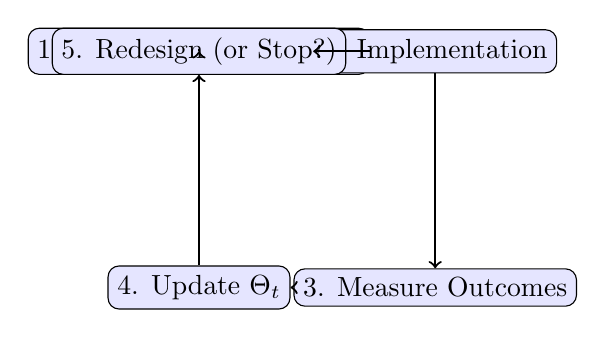
\begin{tikzpicture}[node distance=3cm, auto]
    \node[draw, rounded corners, fill=blue!10] (design) {1. Portfolio Design (Ch20)};
    \node[draw, rounded corners, fill=blue!10, right of=design] (implement) {2. Implementation};
    \node[draw, rounded corners, fill=blue!10, below of=implement] (measure) {3. Measure Outcomes};
    \node[draw, rounded corners, fill=blue!10, left of=measure] (learn) {4. Update $\Theta_t$};
    \node[draw, rounded corners, fill=blue!10, above of=learn] (redesign) {5. Redesign (or Stop?)};

    \draw[->, thick] (design) -- (implement);
    \draw[->, thick] (implement) -- (measure);
    \draw[->, thick] (measure) -- (learn);
    \draw[->, thick] (learn) -- (redesign);
    \draw[->, thick, bend right] (redesign) to (design);
\end{tikzpicture}
\end{center}

\textbf{Question:} When do we stop redesigning? Answer: When learning has \textit{converged}.

\subsection{Convergence Criteria}

Learning has converged when:

\begin{equation}
||\Theta_t - \Theta_{t-1}|| < \epsilon \quad \text{for } T \text{ consecutive periods}
\label{eq:21-convergence}
\end{equation}

Practical values: $\epsilon = 0.05$ (5\% change threshold), $T = 2$ (two periods of stability)

\textbf{Engagement Example (Tech Company):}

\begin{center}
\begin{tabular}{lccc}
\toprule
\textbf{Period} & $E_{\text{max,Autonomy}}$ & $\gamma_{\text{Autonomy,Social}}$ & Converged? \\
\midrule
t=0 (prior) & 0.15 & 0.40 & No \\
t=1 (after 3m) & 0.16 & 0.35 & No \\
t=2 (after 6m) & 0.165 & 0.34 & No \\
t=3 (after 9m) & 0.167 & 0.335 & YES ($\Delta < 0.01$) \\
t=4 (after 12m) & 0.1668 & 0.334 & YES ($\Delta < 0.005$) \\
\bottomrule
\end{tabular}
\end{center}

\textbf{Interpretation:} After 9 months, parameters have stabilized. New learning provides <1\% updates. This is convergence.

\textbf{Decision Rule:}
- If converged: Stop redesigning, maintain current portfolio ($P^*$ is stable)
- If not converged: Continue monitoring, prepare for next redesign

\subsection{Full Engagement Worked Example: Baseline vs Crisis Scenario}

\textbf{Scenario:} Tech company with 500 employees. Goal: Increase engagement from 45\% to 65\%.

\textbf{Baseline (Normal Conditions):}

Portfolio P_baseline:
\begin{itemize}[nosep]
\item Autonomy-supporting feedback (monthly 1:1 conversations focused on autonomy)
\item Peer recognition program (peer-nominated "star performer" awards)
\item Leadership communication (CEO all-hands weekly)
\end{itemize}

Segment-specific baseline effectiveness:
\begin{itemize}[nosep]
\item Autonomy-Seeking segment (30\%): $E_{\text{base}} = 0.20$ (high responsiveness to autonomy cues)
\item Social-Oriented segment (40\%): $E_{\text{base}} = 0.15$ (moderate, peer recognition most effective)
\item Present-Biased segment (30\%): $E_{\text{base}} = 0.12$ (low, needs immediate feedback)
\end{itemize}

Portfolio-level effectiveness:
\begin{equation}
E_{\text{baseline}} = 0.30 \times 0.20 + 0.40 \times 0.15 + 0.30 \times 0.12 = 0.156 \text{ (15.6\% increase)}
\label{eq:21-engagement-baseline}
\end{equation}

\textbf{Crisis Scenario (t=6m):} Company announces layoffs. Context shifts dramatically.

New context:
\begin{itemize}[nosep]
\item Psychological safety drops (fear, uncertainty)
\item Social cohesion weakens (everyone worried about their job)
\item Autonomy-seeking segment becomes risk-averse (wants security, not autonomy)
\end{itemize}

Old portfolio effectiveness COLLAPSES:
\begin{itemize}[nosep]
\item Autonomy-Seeking: $0.20 \to 0.08$ (autonomy cues perceived as loss of support)
\item Social-Oriented: $0.15 \to 0.05$ (peer recognition seen as unfair when layoffs coming)
\item Present-Biased: $0.12 \to 0.04$ (leadership comms trigger anxiety, not motivation)
\end{itemize}

New portfolio-level effectiveness:
\begin{equation}
E_{\text{crisis}} = 0.30 \times 0.08 + 0.40 \times 0.05 + 0.30 \times 0.04 = 0.052 \text{ (5.2\% — COLLAPSE!)}
\end{equation}

\textbf{Redesign Decision:} Crisis triggers immediate portfolio redesign.

\textbf{Crisis Portfolio P_crisis (optimized for psychological safety):}
\begin{itemize}[nosep]
\item Replace autonomy-feedback with safety-assurance (explicit management commitment to job security)
\item Replace peer recognition with team support (collective success framing)
\item Enhance leadership communication (transparency about layoff plans, redeployment support)
\item Add new: Mental health support (counseling, stress management)
\end{itemize}

New crisis effectiveness:
\begin{itemize}[nosep]
\item Autonomy-Seeking: $0.08 \to 0.12$ (safety-assurance helps)
\item Social-Oriented: $0.05 \to 0.14$ (team support resonates)
\item Present-Biased: $0.04 \to 0.09$ (mental health support + transparency helps)
\end{itemize}

New portfolio-level effectiveness:
\begin{equation}
E_{\text{crisis redesigned}} = 0.30 \times 0.12 + 0.40 \times 0.14 + 0.30 \times 0.09 = 0.121 \text{ (12.1\% — RECOVERY!)}
\end{equation}

\textbf{Key Insight:} Despite worse context, redesign recovers from 5.2\% → 12.1\% effectiveness. Same principle as Energia: Context shifts require **qualitative portfolio changes**, not just intensity adjustments.

\textbf{Learning Over Crisis (Parameter Updates):}

\begin{center}
\begin{tabular}{lccccc}
\toprule
\textbf{Phase} & \textbf{Time} & $K^*(t)$ & \textbf{E(P)} & \textbf{Redesign?} & \textbf{Status} \\
\midrule
Baseline & t=0-5m & 3 & 15.6\% & — & Stable \\
Shock & t=6m & 5 & 5.2\% & YES & Crisis detected \\
Adaptation & t=6-9m & 4 & 12.1\% & — & Learning phase \\
Convergence & t=9m+ & 3 & 13.5\% & NO & Stable (converged) \\
\bottomrule
\end{tabular}
\end{center}

\textbf{$K^*(t)$ bei Context-Shock (EIT-EMP-2):} Schock-Faktor $h(\Psi_t) = 1.5$ erhöht $K^*$ temporär von 3 auf 5. Dies erlaubt mehr Interventionen während der Krisenphase (Mental Health Support, Team Support, etc.). Nach Konvergenz sinkt $K^*$ wieder auf 3 (fokussiertes Maintenance-Portfolio).

\textbf{Decision Rule Applied (EIT-EMP-2 Extension):}
\begin{itemize}[nosep]
\item $t=6m$: Context shock detected ($||\Delta \Psi|| > 0.2$) → $K^*(t) \times 1.5$ → Trigger redesign ✓
\item $t=9m$: Learning converged ($\Delta \Theta < 5\%$ for 2 periods) → $K^*(t) \times 0.8$ → Stop redesigning ✓
\item Maintain crisis portfolio P\_crisis until next major context shift
\end{itemize}

\subsection{Comparative Summary: Four Examples Across All Dynamics}

\begin{center}
\begin{tabular}{lccccc}
\toprule
\textbf{Example} & \textbf{Primary Driver} & $K^*$ Range & \textbf{Initial E} & \textbf{After Redesign} & \textbf{Convergence} \\
\midrule
Diabetes & Phase progression & 2→4→3 & 4\% & 18\% & 6-12 months \\
Rente & Policy + Learning & 3→4→3 & 10\% & 12\% & 6-9 months \\
Energia & Context shock & 3→5→3 & 14\%→6\% & 17\% & 3 months \\
Engagement & Psych. shock & 3→5→3 & 15.6\%→5.2\% & 12.1\% & 9 months \\
\bottomrule
\end{tabular}
\end{center}

\textbf{$K^*(t)$ Pattern (EIT-EMP-2):} Alle Beispiele zeigen das gleiche Muster:
\begin{enumerate}[nosep]
\item \textbf{Baseline:} $K^* = 2-3$ (fokussiertes Anfangsportfolio)
\item \textbf{Transition/Shock:} $K^* \uparrow$ auf 4-5 (mehr Interventionen während Anpassung)
\item \textbf{Convergence:} $K^* \downarrow$ auf 3 (refokussiertes Maintenance-Portfolio)
\end{enumerate}

\textbf{Pattern Recognition:}
\begin{itemize}[nosep]
\item All four examples show **redesign increases effectiveness** despite changed conditions
\item Crisis contexts (Energia, Engagement) require fastest redesign (3-6m)
\item Gradual changes (Diabetes phase progression) allow slower redesign (6-12m)
\item Learning convergence typically 6-12 months (2-4 redesign cycles)
\item Decision rule (trigger + convergence criteria) applies to all domains
\end{itemize}

---

\section{Section 5: Synthesis and Bridge to Appendix KKK}
\label{sec:21-synthesis}

\subsection{What This Chapter Provides (Intuitive)}

\begin{tcolorbox}[colback=green!5!white, colframe=green!75!black, title=What Ch21 Answers for Practitioners]

\begin{enumerate}
\item \textbf{When to redesign?} Triggers: Phase change ($\Delta \varphi > 0.3$), Context shock ($||\Delta \Psi|| > 0.2$), Learning update
\item \textbf{How to redesign?} Use Ch20 methods on new $\vec{S}_t$ (phase-affinity, segment multipliers shift)
\item \textbf{How fast does evolution happen?} Depends on phase velocity (empirically calibrated, typically 3-12 months)
\item \textbf{When to stop?} Convergence criteria: Parameter updates plateau ($\Delta \Theta < \epsilon$)
\item \textbf{Multi-period examples:} Diabetes (3 phases), Rente (policy changes), Engagement (learning convergence)
\end{enumerate}

No mathematics beyond basic calculus. Practical decision rules sufficient.

\end{tcolorbox}

\subsection{For Researchers: Formal Mathematical Models in Appendix KKK}

Appendix KKK provides rigorous mathematical treatment:

\begin{itemize}[nosep]
\item \textbf{Section 2:} Phase dynamics as ODE: $d\varphi/dt = v_0 + v_A A_t + v_W W_t$ (derivations, boundary conditions, numerical solutions)
\item \textbf{Section 3:} Context evolution models (linear, nonlinear, with external shocks)
\item \textbf{Section 4:} Bayesian parameter learning (likelihoods, posteriors, convergence rates)
\item \textbf{Section 5:} Optimization with switching costs (Lagrangians, first-order conditions)
\item \textbf{Section 6:} Convergence proofs (fixed points, stability, divergence conditions)
\end{itemize}

\textbf{Reading Guide:}
- Practitioners: Read Ch21 Sections 1-4, skip KKK
- Researchers: Read Ch21 then consult KKK for formal underpinnings
- Implementation teams: Use Ch21 decision rules + decision trees

---

\section{Chapter Overview: Reading Paths}
\label{sec:21-reading-paths}

\begin{tcolorbox}[colback=yellow!5!white, colframe=yellow!75!black, title=Where to Go Next]

\textbf{If you want...} then go to:
\begin{itemize}[nosep]
\item Static portfolio design → Chapter 20 (complete)
\item Dynamic implementation with examples → This chapter (Sections 1-4)
\item Formal mathematics → Appendix KKK (METHOD-DYNAMIC)
\item Parameter sourcing discipline → Appendix JJJ (METHOD-PSG)
\item Applications to specific domains → Chapter 22 (Policy Applications)
\item Moving from design to measurement → Appendix R (Evaluation Protocol)
\end{itemize}

\end{tcolorbox}

---

\subsection{Formal Details}
\label{sec:ch21-formal}

The complete formal treatment appears in Appendix KKK (METHOD-DYNAMIC). Key results:

\begin{itemize}[nosep]
    \item \textbf{Phase Dynamics ODE:} $d\varphi/dt = v_0 + v_A A_t + v_W W_t$ with boundary conditions and numerical solutions
    \item \textbf{Context Evolution:} Linear and nonlinear models with external shock propagation
    \item \textbf{Bayesian Learning:} Likelihood functions, posterior updates, convergence rates for $\Theta_t$
    \item \textbf{Switching Cost Optimization:} Lagrangian formulation for when to redesign portfolios
    \item \textbf{Convergence Proofs:} Fixed point theorems, stability conditions, divergence bounds
\end{itemize}

\subsection{What Comes Next}
\label{sec:ch21-what-comes-next}

\begin{enumerate}
    \item \textbf{Chapter 22 (Policy Applications):} Apply dynamic portfolio framework to real policy domains
    \item \textbf{Chapter 23 (Multi-Level Implementation):} Scale from individual to organizational to national level
    \item \textbf{Appendix KKK:} Full mathematical treatment of all dynamic models
\end{enumerate}

%======================================================================
% SUMMARY SECTION
%======================================================================

\section{Summary}
\label{sec:ch21-summary}

\begin{tcolorbox}[colback=blue!5!white, colframe=blue!75!black,
    title={\textbf{Chapter 21 Summary: Dynamic Portfolio Evolution}}]

\textbf{Core Insight:} Status quo $S_t$ evolves through phase progression, context shifts, and learning updates---requiring systematic portfolio redesign rather than static optimization.

\textbf{Key Results:}
\begin{enumerate}[nosep]
    \item \textbf{Three Evolution Mechanisms:} Phase progression ($\varphi_t$), context shifts ($\Psi_t$), and Bayesian learning ($\Theta_t$)
    \item \textbf{Dynamic $K^*(t)$ (EIT-EMP-2):} Optimale Portfolio-Größe evolviert: $K^*(t) = K^*_0 \cdot g(\varphi_t) \cdot h(\Psi_t) \cdot \ell(\Theta_t)$
    \item \textbf{Redesign Triggers:} Phase change ($\Delta\varphi > 0.3$), context shock ($||\Delta\Psi|| > 0.2$), or significant parameter update
    \item \textbf{$K^*$ Pattern:} Baseline (2-3) → Transition/Shock (4-5) → Convergence (3)
    \item \textbf{Convergence Criteria:} $||\Theta_t - \Theta_{t-1}|| < \epsilon$ for $T$ consecutive periods signals learning completion
    \item \textbf{Four Worked Examples:} Diabetes (phase-driven), Rente (policy-driven), Energia (crisis-driven), Engagement (shock-driven)
\end{enumerate}

\textbf{Transition:} Chapter 22 applies this dynamic framework to real policy domains; Chapter 23 scales implementation across organizational levels.

\end{tcolorbox}

\begin{center}
\textbf{Chapter 11 (EMERGE):} ``How compute optimal intervention profile?'' \\
\textbf{Answer:} EMERGE Algorithm with $K^* = f(\text{budget}, \text{complexity}, \text{stage}, \text{crowding}, \text{scope})$ ✓ \\

\vspace{0.3cm}

\textbf{Chapter 20 asked:} ``Given S_0, what portfolio maximizes E(P|S_0)?'' \\
\textbf{Answer:} Use C1--C7 constraints, optimize via hierarchical workflow. ✓ \\

\vspace{0.3cm}

\textbf{Chapter 21 asks:} ``As S_t evolves, when redesign and when stop?'' \\
\textbf{Answer:} Monitor triggers, recalculate $K^*(t)$, converge when $\Delta\Theta$ plateaus. ✓ \\

\vspace{0.3cm}

\textbf{Together:} EMERGE (Ch11) → Static Portfolio (Ch20) → Dynamic Evolution (Ch21)
\end{center}

%======================================================================
% END OF CHAPTER 21
%======================================================================
